\section{Monitoring}
Il se peut qu'au cours du déploiement d'un site web, celui-ci subisse un temps d'arrêt. Cela signifie que si quelqu'un veut visiter le site, il ne pourra pas le faire. La mise en place d'un outil de monitoring est une tâche primordiale. 
L'outil de monitoring choisit pour ce projet est UpTimeRobot. Il permet de vérifier rapidement si les services sont opérationnels
De plus, cet outil réalise des vérifications de l'état des différents services à des intervalles réguliers. Pour ce projet, l'intervalle choisi est de à 5 minutes étant donné que le site web ne devrait, en aucun cas, subir des interruptions.

\begin{figure}[H]
    \centering
    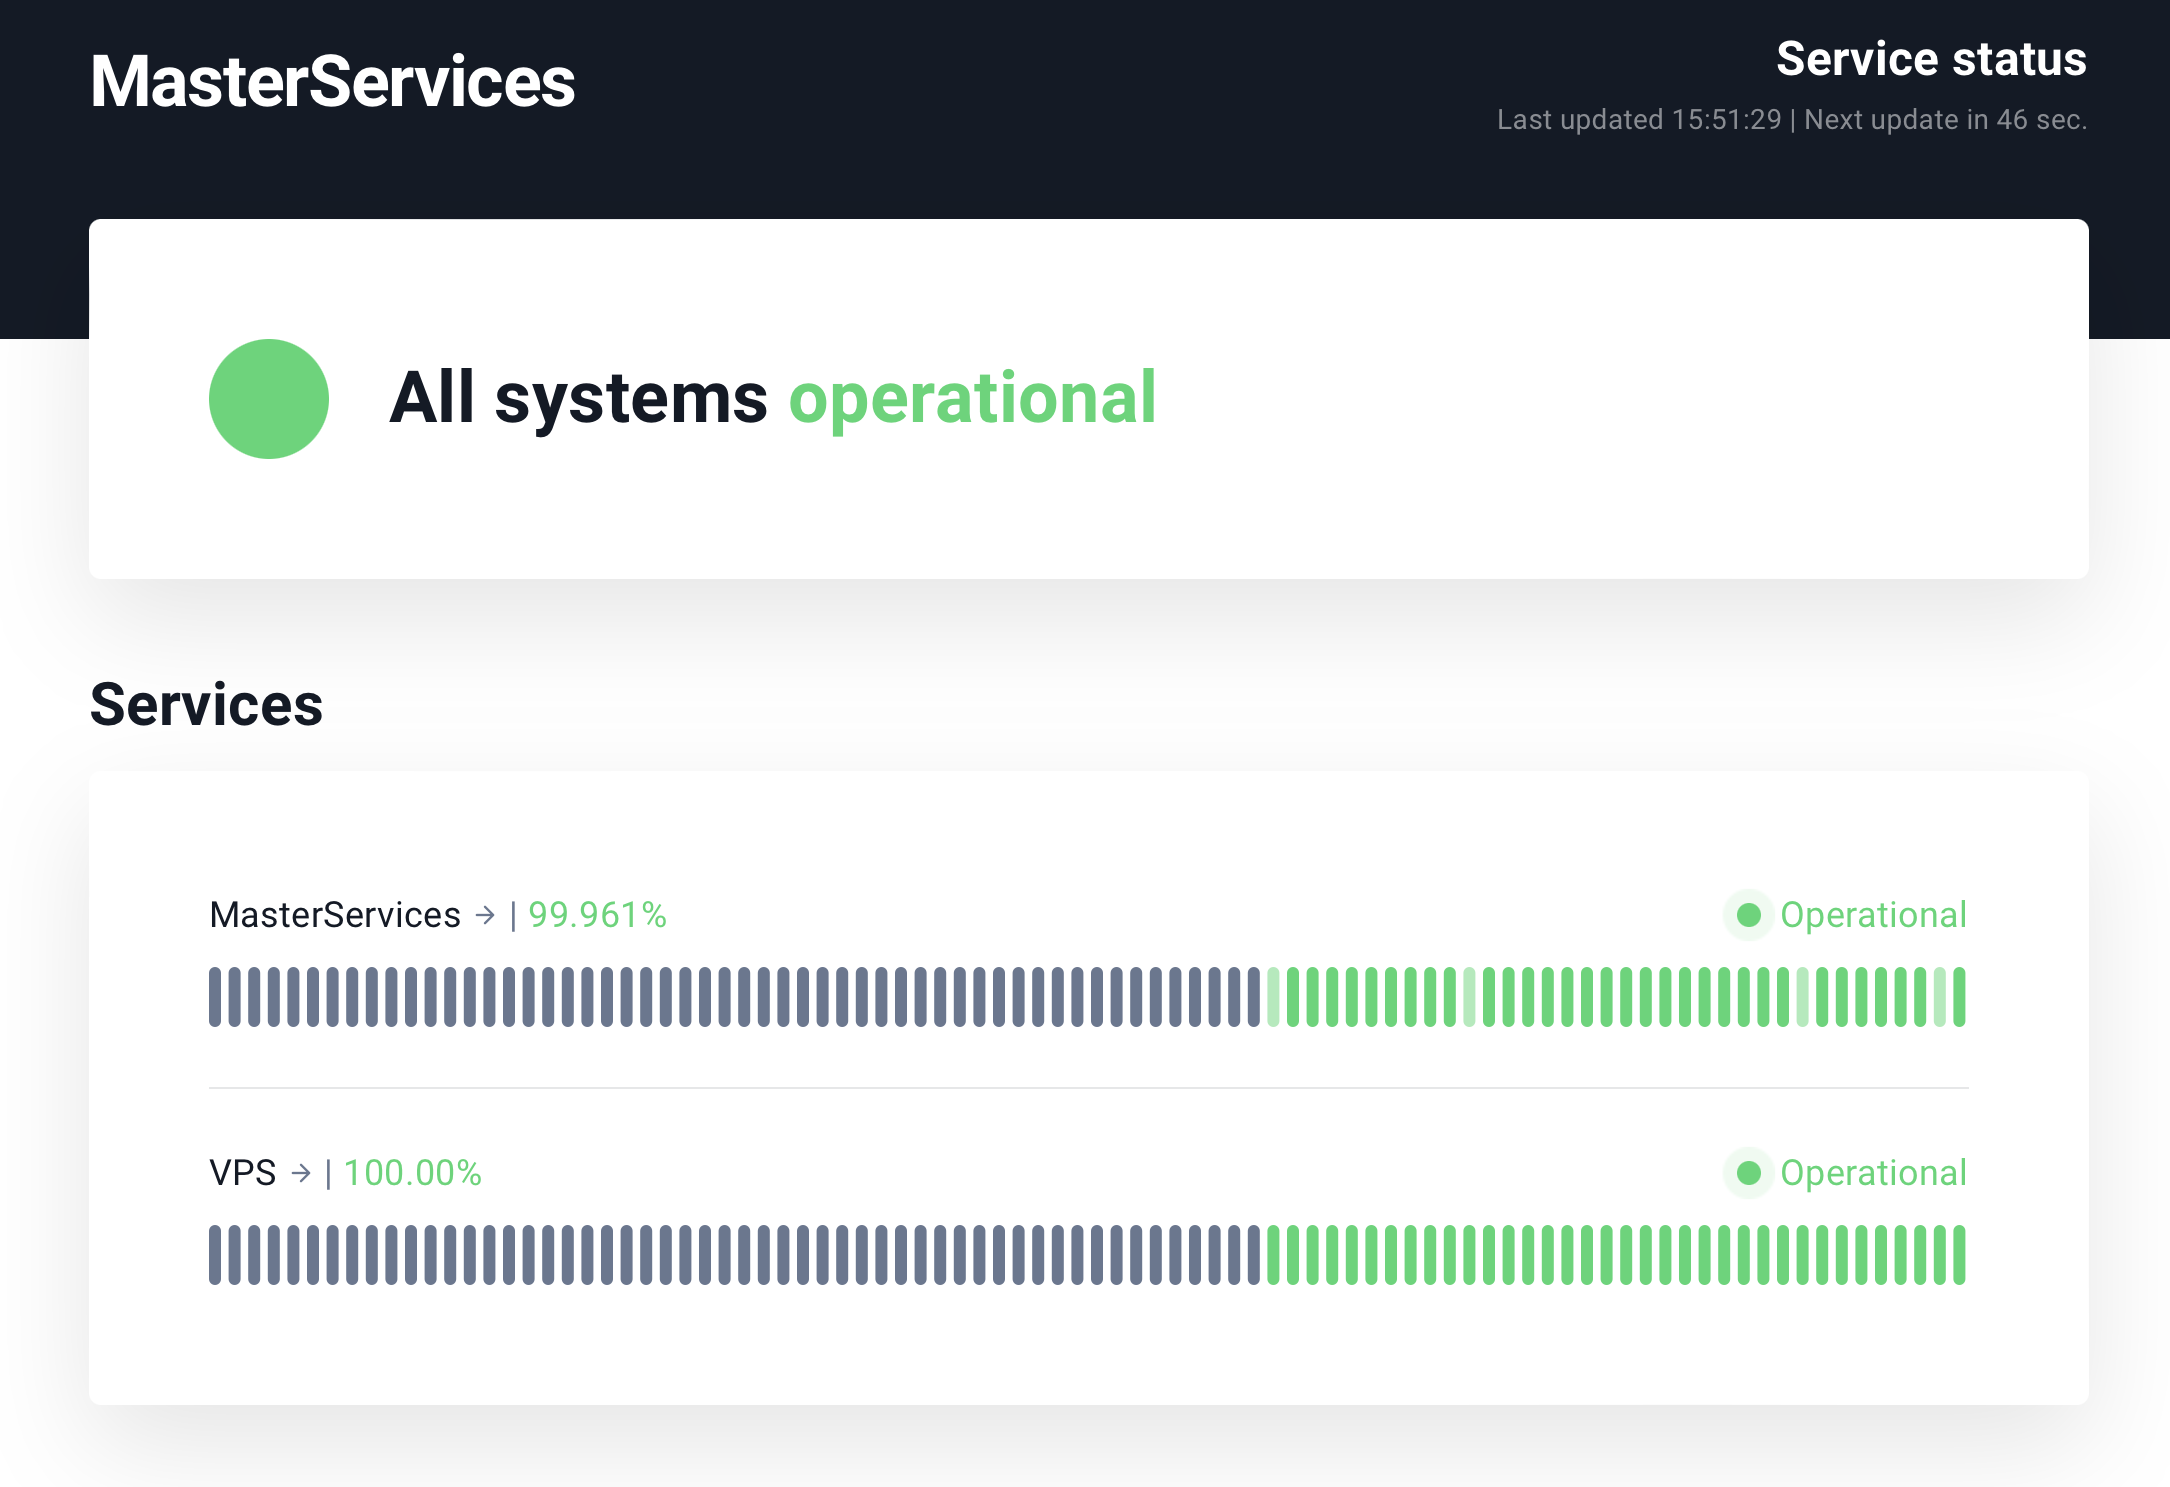
\includegraphics[scale=0.3]{img/uptime.png}
    \caption{Monitoring avec l'outil UpTimeRobot}
    \label{UpTimeRobot}
\end{figure}